\chapter{Software}

All the programs developed, including the Arduino codes, Python script for master interface and template for Web GUI  are available on our \href{https://github.com/Nabla33/Room_Occupancy_Indicating_Network}{GitHub repository}\cite{github}.

\section{Master and Node Codes}

The codes for the master and nodes are written and implemented using Arduino as the networking libraries for the NRF24 are well developed and documented for Arduino based systems.

The program flow is can be depicted by the simple flowcharts as follows.

\subsection{Node}

\begin{center}
	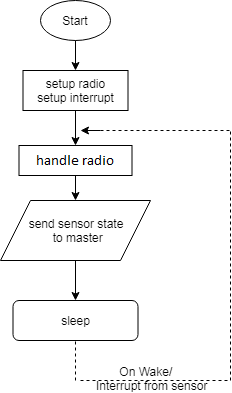
\includegraphics[scale=0.8]{rois_node_flow.png}\\		
	\vspace{10pt}
	Program flow for a sensor node
	
\end{center}

\subsection{Master}

\begin{center}
	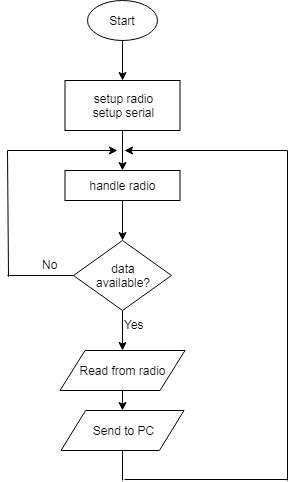
\includegraphics[scale=0.7]{rois_master_flow.png}\\		
	\vspace{10pt}
	Program flow for a the master node
	
\end{center}